\documentclass{ifri}

\setlength{\glsdescwidth}{0.65\textwidth}
% \usepackage{lscape}
\frenchbsetup{StandardLists=true} % à inclure si on utilise \usepackage[french]{babel}
\usepackage{enumitem}

\typeMemoire{Diplôme de Licence en Informatique}
\optionFormation{Sécurité Informatique}
\etudiant{Jospy \textbf{GOUDALO}}
\titreDuMemoire{Prototype d'un syst\`eme de paiement \'electronique des factures d'\'electricit\'e de la SBEE dans un environnement s\'ecuris\'e.}

\dateSoutenance{-}
%\promo{2\up{ème}}
\anneeScolaire{2017-2018}

%%maitre de mémoire
\encadrants{\textbf{Professeur Eugène C. EZIN}\\Enseignant - chercheur en Informatique\\Université d'Abomey-Calavi}

\hypersetup{
 pdftitle={Prototype d'un syst\`eme de paiement \'electronique des factures d'\'electricit\'e de la SBEE dans un environnement s\'ecuris\'e.},
 pdfauthor={Jospy GOUDALO, jospygoudalo@gmail.com},
 pdfsubject={Prototype d'un syst\`eme de paiement \'electronique des factures d'\'electricit\'e de la SBEE dans un environnement s\'ecuris\'e.},
 pdfkeywords={système, paiement, factures, \'electriques, SBEE}
 }

\color{bookColor}

%importation du glossaire
\makeglossaries
\loadglsentries{glossaire/glossaire_reduit}

\begin{document}

\makeatletter
\renewcommand{\thesection}{%
  \ifnum\c@chapter<1 \@arabic\c@section
  \else \thechapter.\@arabic\c@section
  \fi
}
\makeatother



\pageDeGarde
%\pageTitre

\pagecolor{white}

%% page vide
%\thispagestyle{empty}\ \clearpage

\selectlanguage{french}

% sommaire
\pagenumbering{roman}

\tableofcontents
\newpage

%liste des figures
\listoffigures

%liste des tableaux
%\listoftables

%liste des algo
\selectlanguage{french}
%\listofalgorithms

% Les sigles et acronymes
\setglossarystyle{super}
\printglossary[title=Sigles et Abréviations, toctitle=Sigles et Abréviations, type=\acronymtype]

% Le glossaire proprement dit
\setglossarystyle{altlist}
\printglossary[type=main]

%% rdedicaces
\dedicace

\paragraph{}
	\begin{center}
		A    
	\end{center}
	\subparagraph*{\\ \\}
	\begin{center}
	 mon Père  \textbf{Noll GOUDALO} 
	\end{center}
	\begin{center}
    ma Mère  \textbf{Nadine SODEDJI}  
	\end{center}
	\begin{center}
      et mon Frère \textbf{Brice GOUDALO}
	\end{center}


 

%% remerciements
\remerciements


\paragraph{}
      Nous exprimons notre vive gratitude aux personnes physiques et institutions qui ont contribué à rendre meilleur notre travail,
   notamment :
  \begin{itemize}
   \item M. Eugène C. EZIN,  notre Maître de mémoire et Directeur de l'Institut de Formation et de Recherche en Informatique (IFRI);
   \item M. Armand ACCROMBESSI, D\'eveloppeur et enseignant à l'IFRI;
   \item Tous les enseignants de l'IFRI pour nous avoir donn\'e les enseignements n\'ecessaires tout au long de notre formation;
   \item M. Camille METINHOUE, Directeur des Syst\`emes d'Information de la SBEE;
   \item M. Idriss SANTANNA et M. Arron ALLADAYE, mes encadreurs  de stage respectivement Chef Service Syst\`eme, S\'ecurit\'e et Maintenance des Infrastructures et Chef Service R\'eseaux T\'el\'ecommunications et TIC \`a la  Direction des Syst\`emes d'Information de la SBEE;
   \item Tout ceux du personnel de la SBEE qui nous ont apport\'es leur soutien tout au long de notre stage;
  \end{itemize}
    Que tous ceux qui nous ont aidé, de près ou de loin, trouvent ici l'expression de nos sentiments les meilleurs.

%\newpage

% Résume
\resume
\selectlanguage{french}
\begin{abstract}
Resume en francais

\paragraph{}
\textbf{Mots clés}: s\'ecurit\'e ,paiement, factures, sbee, 
\end{abstract}

\newpage
\selectlanguage{english}
\begin{abstract}

Resume en anglais

\paragraph{}
\textbf{Key words}: ....,....,....
\end{abstract}





\pagenumbering{arabic}
\setcounter{page}{1}
%%introduction
\introduction
    \paragraph{}
      \small{
      L'informatique, science du traitement rationnel et automatisé de l'information, est devenue aujourd'hui un outil indispensable pour l'évolution de toute nation, de toute société. Elle est passée d'un statut luxueux à un statut nécessaire. La preuve : toute structure de renom investit un budget non n\'egligeable pour l'informatisation de ses opérations. Cependant, certains sont ne sont toujours pas en phase avec l'\'evolution de la technologie en rapport avec les services qu'ils offrent et la s\'ecurit\'e de ces derni\`eres. Dans le m\^eme temps, des individus profitent de ce ph\'enom\`ene pour pi\'eger les autres ignorant le fonctionnement de l'ordinateur ou non dans le but de voler ou alt\'erer des informations précieuses et confidentielles pour des fins diverses : c'est la cybercriminalité. Vu l'ampleur que prend ces diff\'erents crimes, il devient n\'ecessaire de voir autrement l'importance de la s\'ecurit\'e dans tous les syst\`emes d'informations.
    
    \section{Contexte et justification}
    
	Le Bénin s’inscrit depuis quelques années dans une politique de restructuration du secteur numérique pour y insuffler une nouvelle dynamique. Plusieurs projets et programmes sont donc nés de cette volonté et constituent une feuille de route pour les acteurs au cœur de cette restructuration. 
	\\Dans l'optique de contribuer au d\'eveloppement de ce secteur et surtout de faciliter la vie \`a la population b\'eninoise, nous avons pens\'e \`a mettre en place une plateforme permettant le paiement \`a distance des factures d'\'electricit\'e de la SBEE. Cependant, il s'agit d'un syst\`eme assez critique lorsque nous consid\'erons la quantit\'e et la criticit\'e/le caractère critique  du flux d'informations que nous aurons \`a traiter. La sécurité de l'information revêtant une importance capitale pour la survie d'un peuple, il faudra aussi mettre en oeuvre un système de défense face aux menaces pour réduire l'impact des attaques et essayer, au maximum, d'éliminer les risques. Un aucun aspect ne doit \^etre pris \`a la l\'eg\`ere.
	}
    
    \section{Problématique}
    \small{
	Il n'est plus \`a d\'emontrer que l'\'electricit\'e est \`a la base de tout d\'eveloppement. De la disponibilité de l’énergie dépend la satisfaction de tous les besoins humains fondamentaux : l’eau, l’alimentation, la santé, l’éducation. L'option la plus accessible est de souscrire \`a un abonnement post-pay\'e avec la SBEE.
	N\'eanmoins il n'est pas rare de constater qu'apr\`es de longues heures d'attente au guichet de la SBEE, l'on vous dise: ``D\'esol\'e monsieur nous avons un probl\`eme de connexion. Veuillez repasser demain.''. Il faudra donc repasser plus tard pour solder la facture alors que nous n'avons pas forc\'ement assez de temps pour cela. \\
	Nous sommes aussi parfois confront\'es \`a l'oubli des factures non pay\'ees. Cependant quand vous n'\^etes pas \`a jour apr\`es un d\'elai d'environ un mois, un agent peut passer \`a tout moment couper le courant et vous devez payer des p\'enalit\'es. Notre travail consistera donc \`a mettre en place une application web permettant le paiement des factures depuis un t\'el\'ephone portable ou un ordinateur connect\'e \`a Internet. Cependant les donn\'ees g\'erees par cette application sont sensibles et critiques. A titre d'exemple les informations de votre carte VISA\footnote{Carte de paiement émise par l'établissement bancaire de son titulaire} pourraient \^etre vol\'ees. La carte sera donc utilis\'ee \`a votre insu et votre argent ne vous appartiendra plus. Il sera donc nécessaire de prendre en compte toutes les menaces possibles et d'y apporter des solutions efficientes. Ainsi nous pourrions avoir une application s\'ecuris\'ee permettant le paiement des factures \'electriques depuis un appareil connect\'e \`a Internet.
	}

    \section{Objectifs}
    \small{ 
	  Notre projet a pour objectif principal de faciliter le paiement des factures \'electriques de la SBEE et de mettre en place les garde four nécessaire pour réduire les attaques informatiques.
	        
	  Plus précisément, il s'agira de :
	
    \begin{itemize}
	\item Rappeler aux personnes utilisant la plateforme qu'ils ont des impay\'es (via des SMS et/ou des emails)
        \item Assurer la disponibilit\'e compl\`ete de la plateforme afin que les consultations et paiements puissent se faire \`a n'importe quel moment.
	\item Garantir la s\'ecurit\'e de toutes les transactions financi\`eres effectu\'ees via la plateforme
	\item Construire un historique afin d'avoir une trace des factures pay\'ees et impay\'ees ainsi que des d\'epenses.
    \end{itemize}
    }

    \section{Environnement de stage}
      \small{
	Ce travail \`a \'et\'e r\'ealis\'e dans les locaux de la Direction des Syst\`emes Informatiques (DSI) de la Soci\'et\'e B\'eninoise d'Energie Electrique (SBEE) - Direction G\'en\'erale. La SBEE a pour mission de produire, de transporter et de distribuer l’énergie électrique sur l’ensemble du territoire national. Elle a son siège social à Cotonou - Ganhi et couvre le territoire national à travers  huit (8) Directions Régionales et trente-neuf (39) agences géographiquement réparties dans tous les départements du pays.
      }
      
    \section{Organisation du mémoire}
	\small{
	  Le présent travail se présente en trois (03) chapitres. Le premier concerne la revue de littérature sur le syst\`eme existant (actuel) permettant le paiement des factures et quelques notions par rapport \`a la s\'ecurit\'e des applications Web. Le deuxième chapitre aborde les choix organisationnels (proc\'edures) et techniques opérés en vue de la conception et de la réalisation des solutions proposées. Le troisième chapitre, quant à lui, fait une analyse critique des résultats issus de nos tests après les avoir exposés.
	}



%\lhead[]{} \rhead[]{} \chead[]{}
\selectlanguage{french}
\fancyhead[L]{\tiny \leftmark}
\fancyhead[R]{\scriptsize \rightmark}
\fancyfoot[C]{\thepage}


\chapter{Revue de littérature}\label{chap:1}
    \section*{Introduction}
	\paragraph{}
      Pour bien réaliser un projet, un état des lieux permettant de faire un point sur le sujet du projet est requis. Ainsi, ce chapitre présente un état des lieux concernant les intrusions informatiques. Dans un premier temps, nous aborderons les généralités sur les intrusions informatiques, puis nous présenterons quelques solutions existantes.
  \section{Gd'Or}
    \paragraph{}
  Informations receuillies par rapport \`a Gd'or.
  
  \begin{itemize}
    \item Gestion Clientele Electricit\'e et/ou Eau
    \item Comptabilit\'e G\'en\'erale, Analytique, Budg\'etaire
    \item Paie et G
    estion des Ressources Humaines
    \item Gestion des stocks
    \item Gestion des Approvisionnements
    \item Immobilisations
    \item Mon\'etique
  \end{itemize}
  \section{S\'ecurit\'e des applications Web}
    \paragraph{}
  Au siècle de l'information, la cyber-sécurité est un défi omniprésent. Les attaques peuvent cibler n'importe quel site internet pour un nombre croissant de raisons. Un manque de sécurité dans une application peut causer des dysfonctionnements, des arrêts complets de service ainsi que des pertes de données dommageables pour les utilisateurs et l'image de l'entreprise. Pour s'en prémunir, les entreprises doivent mettre en place des mesures de sécurité strictes dans le processus de développement d'applications Web. \\
  Cette section expose quelques failles de s\'ecurit\'e li\'ees aux applications web et quelques bonnes pratiques pour rem\'edier.
  
\subsection{Notion de hacker et de cracker}
  \paragraph{}
    Un hacker est une personne qui, par jeu, goût du défi ou souci de notoriété, cherche à contourner les protections d'un logiciel, à s'introduire frauduleusement dans un système ou un réseau informatique. \cite{A} \footnote{Recommandation officielle : fouineur.}.\\Un cracker, quant à lui, s’introduit tout aussi frauduleusement dans un système informatique pour en entraver ou en fausser le fonctionnement. Son action est souvent plus dévastatrice.
	

\subsection{Mode opératoire d'une attaque informatique}
  \paragraph{}
    Une attaque informatique peut être décomposé en une suite d’étapes ou phases. Lorsqu’elles sont réunies, ces étapes forment une méthodologie complète pour mener à bien une attaque informatique. L’établissement d’une méthodologie permet de décomposer une procédure complexe en une suite de tâches gérables de taille plus réduite. Ainsi nous regroupons cette méthodologie en quatre étapes qui sont \textbf{la reconnaissance}, \textbf{les scans}, \textbf{l'exploitation}, \textbf{la post-exploitation et le maintien d'accès} \footnote{La post exploitation et le maintien d'accès forment une étape.}\cite{c}.
      
  \subsubsection{La reconnaissance}
    \paragraph{}
      La reconnaissance, ou recueil d’informations, est probablement la plus importante des quatre phases. Plus le hacker passe du temps à collecter des informations sur sa cible, plus les phases suivantes auront une chance de réussir\cite{c}. En effet la reconnaissance permet de connaitre la cible dans les détails, de connaître les points forts et surtout les points faibles afin de notifier les prochaines possibilités d'attaque.

  \subsubsection{Les scans}
    \paragraph{}
      Les scans sont des procédés ayant pour objectif d’identifier les systèmes actifs et les services qui existent sur les systèmes scannés. Dans ce cadre, l'hacker prend le soin de vérifier l'activité d'un système, de trouver les portes ouvertes (les ports), de vérifier les processus tournant sur le système et d'aller à la recherche des vulnérabilités. Ce stade requiert une compréhension plus avancée des systèmes informatiques pour mieux comprendre les résultats recueillis \footnote{Informations recueillis au cours du scan}\cite{c}.
      
  \subsubsection{L'exploitation}
    \paragraph{}
      En termes simples, l’exploitation consiste à obtenir un contrôle sur un système. Toutefois, il est à notifier que tout exploit ne conduit pas à la compromission intégrale d’un système. Un hacker peut se servir donc d'un exploit pour télécharger des contenus dont il ne détient pas la propriété pendant qu'un autre utilise un exploit pour crypter les fichiers du système. L'utilisation de l'un des exploits \footnote{Un exploit est le moyen par lequel un attaquant, ou un pentester en l’occurrence, profite d’un défaut dans un système, une application ou un service.} dépend donc de l'objectif visé par l'hacker \cite{E}.

  \subsubsection{Post exploitation et maintien d’accès}
    \paragraph{}
      Cette étape consiste à couvrir les traces de l'intrus agissant afin de ne pas se faire repérer \cite{E}. Il permet aussi à ce dernier de faciliter ses prochains accès à la machine victime de ses attaques par l'installation de portes dérobées communément appelées "Backdoor". Ainsi, il n'aura plus besoin de reprendre toutes les étapes de son processus pour accéder à la machine dont il prend le contrôle.\\ \\
      

\begin{figure}[H]
  \begin{center}
    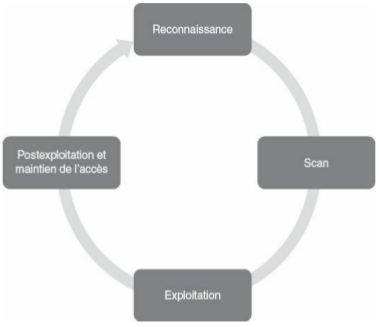
\includegraphics[scale=0.5]{images/zeh_cycle.png}
  \end{center}
  \caption[Représentation cyclique de la méthodologie ZEH.]
    {Méthodologie ZEH, Patrcick Engebretson, "Les bases du hacking", PEARSON 2013}
    \label{Methodologie d'intrusion}
\end{figure}


\paragraph{}
  La méthodologie d'attaque étant cernée, nous allons maintenant présenter les différentes failles auxquelles sont expos\'ees les applications web.	    
		    

\subsection{Menaces et risques applicatifs}
  \subsubsection{Failles de Sécurité}
    \paragraph{}
    Le projet OWASP (Open Web Application Security Project) est une communauté ouverte destinée à permettre aux organisations de développer, d'acheter et de gérer des applications et des API fiables. Tous les outils, documents, vidéos, présentations et chapitres OWASP sont gratuits et ouverts à toute personne intéressée par l'amélioration de la sécurité des applications. L'approche de la sécurité des applications en tant que problème de personnes, de processus et de technologie est  préconis\'ee, car les approches les plus efficaces en matière de sécurité des applications nécessitent des améliorations dans ces domaines. OWASP produit aussi de nombreux types de matériaux de manière collaborative, transparente et ouverte. Le projet soutient la recherche innovante en matière de sécurité avec des subventions et des infrastructures.
    
    \paragraph{}
    L'OWASP Top 10 est un document de sensibilisation puissant pour la sécurité des applications Web. Il représente un large consensus sur les risques de sécurité les plus critiques pour les applications Web. Les membres du projet incluent une variété d'experts en sécurité du monde entier qui ont partagé leur expertise pour produire cette liste.
    Nous recommandons \`a toutes les entreprises d'adopter ce document de sensibilisation au sein de leur organisation et de commencer à faire en sorte que leurs applications Web minimisent ces risques. L'adoption du Top 10 de l'OWASP est peut-être la première étape la plus efficace pour changer la culture de développement de logiciels au sein de votre organisation en une culture qui produit du code sécurisé.
    \paragraph{}
    Cette mise à jour majeure (celle de 2017) ajoute plusieurs nouveaux problèmes, dont deux problèmes sélectionnés par la communauté - \textbf{A8: 2017 - Dés\'erialisation non sécurisée} et \textbf{A10: 2017 - Insuffisance de Logs et de Surveillance}. Les deux principales différences par rapport aux versions précédentes du Top 10 d'OWASP sont les retours substantiels de la communauté et les données complètes rassemblées par des dizaines d'organisations, probablement la plus grande quantité de données jamais rassemblées dans la préparation d'une norme de sécurité applicative. Cela nous permet de croire que le nouveau Top 10 d'OWASP aborde les risques de sécurité applicative les plus importants auxquels sont confrontées les entreprises.
    \paragraph{}
    L'un des principaux objectifs du Top 10 d'OWASP est d'éduquer les développeurs, les concepteurs, les architectes, les gestionnaires et les organisations sur les conséquences des faiblesses les plus courantes et les plus importantes de la sécurité des applications Web. Le Top 10 fournit des techniques de base pour se protéger contre ces zones problématiques à haut risque et fournit des indications sur les endroits où aller.
    \paragraph{}
    Les attaquants peuvent potentiellement utiliser de nombreux chemins différents à travers votre application pour nuire à votre entreprise ou organisation. Chacun de ces chemins représente un risque qui peut ou non être suffisamment sérieux pour justifier une attention. Parfois, ces chemins sont triviaux à trouver et à exploiter, et parfois ils sont extrêmement difficiles. De même, le préjudice causé peut être sans conséquence, ou vous mettre à la faillite. Pour déterminer le risque pour votre organisation, vous pouvez évaluer la probabilité associée à chaque agent de menace, vecteur d'attaque et faiblesse de la sécurité et le combiner avec une estimation de l'impact technique et commercial sur votre organisation. Ensemble, ces facteurs déterminent votre risque global.
    
    \subsubsection{OWASP Top 10 - 2017}
      \paragraph{}
      Le rapport « OWASP Top 10 » permet ainsi à l’équipe projet de se focaliser sur la protection de l’application Web
      face aux menaces les plus importantes, ce qui est moins couteux et plus facilement réalisable
      que d’essayer de se protéger de tous les dangers. L’OWASP établit le classement 2017
      ci-dessous, dont chacune des failles est développée dans les chapitres suivants :
            
  \begin{enumerate}
	\vspace*{0.8cm} \item \textbf{Injection} \vspace*{-0.4cm}
	\paragraph{}
	Des erreurs d'injection, telles que l'injection SQL, NoSQL, OS et LDAP, se produisent lorsque des données non fiables sont envoyées à un interpréteur dans le cadre d'une commande ou d'une requête. Les données hostiles de l'attaquant peuvent amener l'interpréteur à exécuter des commandes inattendues ou à accéder aux données sans autorisation appropriée.
	\paragraph{}L'injection peut parfois conduire à une prise en charge complète de l'hôte. L'impact métier dépend des besoins de l'application et des données.
	\paragraph{}La prévention de l'injection nécessite de séparer les données des commandes et des requêtes. L'option préférée consiste à utiliser une API sécurisée, qui évite l'utilisation complète de l'interpréteur ou fournit une interface paramétrée, ou migre pour utiliser les outils ORC (Object Relational Mapping Tools)

	\vspace*{0.8cm} \item \textbf{Authentification brisée} \vspace*{-0.4cm}
	\paragraph{}
	Les fonctions d'application liées à l'authentification et à la gestion de session sont souvent incorrectement implémentées, permettant aux pirates de compromettre les mots de passe, clés ou jetons de session ou d'exploiter d'autres failles d'implémentation pour prendre temporairement ou définitivement les identités des autres utilisateurs.
	La prévalence de l'authentification brisée est généralisée en raison de la conception et de la mise en œuvre de la plupart des contrôles d'identité et d'accès. La gestion de session est le fondement des contrôles d'authentification et d'accès et est présente dans toutes les applications avec état.
	\paragraph{}
	Les attaquants doivent avoir accès à seulement quelques comptes ou à un seul compte admin pour compromettre le système. Selon le domaine de l'application, cela peut permettre le blanchiment d'argent, la fraude à la sécurité sociale et le vol d'identité, ou divulguer des informations hautement sensibles protégées par la loi.
	\paragraph{}
	Lorsque cela est possible, implémentez l'authentification multi-facteur pour éviter les attaques automatisées, le bourrage des informations d'identification, la force brute et la réutilisation des informations d'identification volées. Ne pas envoyer ou déployer avec des informations d'identification par défaut, en particulier pour les utilisateurs d'administration.
	
	\vspace*{0.8cm} \item \textbf{Exposition de données sensibles} \vspace*{-0.4cm}
	\paragraph{}
	De nombreuses applications Web et API ne protègent pas correctement les données sensibles, telles que les données financières, les soins de santé et les informations personnelles. Les attaquants peuvent voler ou modifier de telles données faiblement protégées pour effectuer une fraude par carte de crédit, un vol d'identité ou d'autres crimes. Les données sensibles peuvent être compromises sans protection supplémentaire, telles que le cryptage au repos ou en transit, et nécessitent des précautions spéciales lors d'un échange avec le navigateur.
	\paragraph{}
	Au cours des dernières années, cela a été l'attaque la plus courante. La faille la plus fréquente est simplement de ne pas chiffrer les données sensibles. Lorsque la cryptographie est utilisée, la génération et la gestion de clés faibles et la faible utilisation d'algorithmes, de protocoles et de chiffrements sont courants, en particulier pour les techniques de stockage de hachage avec mot de passe faible. 
	Généralement, ces informations incluent des informations personnelles sensibles telles que des dossiers médicaux, des informations d'identification, des données personnelles et des cartes de crédit, qui nécessitent souvent une protection telle que définie par les lois ou réglementations telles que le GDPR UE ou les lois locales sur la confidentialité.
	\paragraph{}
	Classer les données traitées, stockées ou transmises par une application. Identifiez les données sensibles en fonction des lois sur la confidentialité, des exigences réglementaires ou des besoins de l'entreprise.
	Appliquer les contrôles selon la classification.

	\vspace*{0.8cm} \item \textbf{Entités externes XML (XXE)} \vspace*{-0.4cm}
	\paragraph{}
	De nombreux processeurs XML anciens ou mal configurés évaluent les références d'entités externes dans les documents XML. Les entités externes peuvent être utilisées pour divulguer des fichiers internes à l'aide du gestionnaire d'URI de fichier, des partages de fichiers internes, de l'analyse de port interne, de l'exécution de code à distance et des attaques par déni de service.
	\paragraph{}
	Par défaut, de nombreux processeurs XML plus anciens permettent la spécification d'une entité externe, un URI qui est déréférencé et évalué pendant le traitement XML. 
	Ces failles peuvent être utilisées pour extraire des données, exécuter une requête à distance à partir du serveur, analyser des systèmes internes, effectuer une attaque par déni de service et exécuter d'autres attaques.
	\paragraph{}
	Autant que possible, utilisez des formats de données moins complexes tels que JSON et évitez la sérialisation des données sensibles.
	Corrigez ou mettez à niveau tous les processeurs et bibliothèques XML utilisés par l'application ou sur le système d'exploitation sous-jacent.

	\vspace*{0.8cm} \item \textbf{Contrôle d'accès brisé} \vspace*{-0.4cm}
	\paragraph{}
	Les restrictions sur ce que les utilisateurs authentifiés sont autorisés à faire ne sont souvent pas correctement appliquées. Les attaquants peuvent exploiter ces failles pour accéder à des fonctionnalités et / ou données non autorisées, telles que l'accès aux comptes d'autres utilisateurs, l'affichage de fichiers sensibles, la modification des données d'autres utilisateurs, la modification des droits d'accès, etc.
	\paragraph{}
	Les faiblesses du contrôle d'accès sont courantes en raison du manque de détection automatisée et du manque de tests fonctionnels efficaces par les développeurs d'applications. 
	L'impact technique est celui des attaquants agissant en tant qu'utilisateurs ou administrateurs, ou des utilisateurs utilisant des fonctions privilégiées, ou créant, accédant, mettant à jour ou supprimant chaque enregistrement.
	\paragraph{}
	Le contrôle d'accès n'est efficace que s'il est appliqué dans un code côté serveur approuvé ou dans une API sans serveur, où l'attaquant ne peut pas modifier la vérification du contrôle d'accès ou les métadonnées.
	À l'exception des ressources publiques, refus par défaut.
	Implémentez les mécanismes de contrôle d'accès une fois et réutilisez-les dans toute l'application, y compris en minimisant l'utilisation de CORS.

	\vspace*{0.8cm} \item \textbf{Mauvaise configuration de la sécurité} \vspace*{-0.4cm}
	\paragraph{}
	La mauvaise configuration de la sécurité est le problème le plus souvent rencontré. Ceci est généralement le résultat de configurations par défaut non sécurisées, de configurations incomplètes ou ad hoc, d'un stockage cloud ouvert, d'en-têtes HTTP mal configurés et de messages d'erreur détaillés contenant des informations sensibles. Non seulement tous les systèmes d'exploitation, cadres, bibliothèques et applications doivent être configurés de manière sécurisée, mais ils doivent également être corrigés / mis à niveau en temps opportun.
	\paragraph{}
	Une mauvaise configuration de sécurité peut se produire à n'importe quel niveau d'une pile d'application, notamment les services réseau, la plateforme, le serveur Web, le serveur d'applications, la base de données, les frameworks, le code personnalisé et les machines virtuelles pré-installées.
	De telles failles donnent souvent aux attaquants un accès non autorisé à certaines données ou fonctionnalités du système. Parfois, de tels défauts entraînent un compromis complet du système.
	\paragraph{}
	Des processus d'installation sécurisés devraient être mis en œuvre. Par exemple, un processus de renforcement répétable qui permet de déployer rapidement et facilement un autre environnement correctement verrouillé. Les environnements de développement, d'assurance qualité et de production doivent tous être configurés de manière identique, avec des informations d'identification différentes utilisées dans chaque environnement. Ce processus devrait être automatisé pour minimiser les efforts requis pour installer un nouvel environnement sécurisé.

	\vspace*{0.8cm} \item \textbf{Cross-Site Scripting (XSS)} \vspace*{-0.4cm}
	\paragraph{}
	Les failles XSS se produisent chaque fois qu'une application inclut des données non fiables dans une nouvelle page Web sans validation ou échappée, ou met à jour une page Web existante avec des données fournies par l'utilisateur en utilisant une API de navigateur pouvant créer du code HTML ou JavaScript. XSS permet aux attaquants d'exécuter des scripts dans le navigateur de la victime, ce qui peut détourner des sessions utilisateur, dégrader des sites Web ou rediriger l'utilisateur vers des sites malveillants.
	XSS est le deuxième problème le plus répandu dans le Top 10 d'OWASP, et se retrouve dans environ deux tiers de toutes les applications.
	\paragraph{}
	L'impact de XSS est modéré pour XSS réfléchi et DOM XSS, et sévère pour XSS stocké, avec l'exécution de code à distance sur le navigateur de la victime, comme voler des informations d'identification, des sessions, ou livrer des logiciels malveillants à la victime.
	\paragraph{}
	La prévention de XSS nécessite la séparation des données non fiables du contenu du navigateur actif. Cela peut être réalisé en utilisant des frameworks qui échappent automatiquement à XSS par conception, comme le dernier Ruby on Rails, React JS. Apprenez les limites de la protection XSS de chaque framework et gérez correctement les cas d'utilisation qui ne sont pas couverts. L'échappement de données de requête HTTP non fiables en fonction du contexte de la sortie HTML (corps, attribut, JavaScript, CSS ou URL) résoudra les vulnérabilités XSS Reflected\footnote{courte definition ici} et Stored\footnote{courte definition ici}.
	
	\vspace*{0.8cm} \item \textbf{Désérialisation non sécurisée} \vspace*{-0.4cm}
	\paragraph{}
	La désérialisation non sécurisée conduit souvent à l'exécution de code à distance. Même si les failles de désérialisation n'aboutissent pas à l'exécution de code à distance, elles peuvent être utilisées pour effectuer des attaques, y compris des attaques de relecture, d'injection et d'escalade de privilèges.
	\paragraph{}
	Certains outils peuvent détecter des défauts de désérialisation, mais une assistance humaine est souvent nécessaire pour valider le problème.
	L'impact des défauts de désérialisation ne peut pas être surestimé. Ces failles peuvent mener à des attaques d'exécution de code à distance, l'une des attaques les plus graves possibles.
	\paragraph{}
	Le seul modèle architectural sûr est de ne pas accepter les objets sérialisés provenant de sources non fiables ou d'utiliser des supports de sérialisation qui autorisent uniquement les types de données primitifs. Si cela n'est pas possible, il faut faire une implémentation de contrôles d'intégrité tels que les signatures numériques sur tous les objets sérialisés pour empêcher la création d'objets hostiles ou la falsification de données.

	\vspace*{0.8cm} \item \textbf{Utilisation de composants avec des vulnérabilités connues} \vspace*{-0.4cm}
	\paragraph{}
	Les composants, tels que les bibliothèques, les frameworks et autres modules logiciels, fonctionnent avec les mêmes privilèges que l'application. Si un composant vulnérable est exploité, une telle attaque peut faciliter la perte de données sérieuse ou la prise de contrôle du serveur. Les applications et les API utilisant des composants présentant des vulnérabilités connues peuvent compromettre les défenses de l'application et permettre diverses attaques et impacts.
	\paragraph{}
	La prévalence de ce problème est très répandue. Les modèles de développement à forte composante peuvent amener les équipes de développement à ne plus comprendre quels composants ils utilisent dans leur application ou leur API, et encore moins les tenir à jour. 
	Bien que certaines vulnérabilités connues n'entraînent que des impacts mineurs, certaines des violations les plus importantes à ce jour reposent sur l'exploitation de vulnérabilités connues dans les composants. Selon les actifs que vous protégez, ce risque devrait peut-être figurer en tête de liste.
	\paragraph{}
	Un processus de gestion des correctifs devrait être en place pour supprimez les dépendances non utilisées, les fonctions inutiles, les composants, les fichiers et la documentation.
	Abonnez-vous à des alertes par e-mail pour connaître les failles de sécurité liées aux composants que vous utilisez.
	N'obtenez que des composants de sources officielles sur des liens sécurisés. Préférer les packages signés pour réduire les risques d'inclusion d'un composant malveillant modifié.

	\vspace*{0.8cm} \item \textbf{Insuffisance de Logs et de Surveillance} \vspace*{-0.4cm}
	\paragraph{}
	Une journalisation et une surveillance insuffisantes, couplées à une intégration manquante ou inefficace avec la réponse aux incidents, permettent aux attaquants d'attaquer davantage les systèmes, de maintenir la persistance, de pivoter vers plus de systèmes et d'altérer, extraire ou détruire des données. La plupart des études de violation montrent que le temps de détection d'une violation dépasse 200 jours, généralement détectés par des parties externes plutôt que par des processus internes ou de surveillance.
	\paragraph{}
	Une stratégie pour déterminer si vous avez une surveillance suffisante est d'examiner les journaux après les tests de pénétration. Les actions des testeurs doivent être enregistrées suffisamment pour comprendre les dommages qu'ils ont pu infliger.
	La plupart des attaques réussies commencent par un sondage de vulnérabilité. Permettre de telles sondes de continuer peut augmenter la probabilité d'exploitation réussie à près de 100\%.
	\paragraph{}
	En fonction du risque de stockage ou de traitement des données par l'application:
	Assurez-vous que tous les échecs de connexion, de contrôle d'accès et de validation des entrées côté serveur peuvent être consignés avec un contexte utilisateur suffisant pour identifier les comptes suspects ou malveillants, et conservés suffisamment longtemps pour permettre une analyse légale retardée.
	Assurez-vous que les journaux sont générés dans un format pouvant être facilement utilisé par des solutions de gestion de journaux centralisées.	
      \end{enumerate}

      \subsection{Quelques bonnes pratiques}
      \paragraph{}
	\underline{a confir\`mer}
	Parler des bonnes pratiques lors du developpement. Utiliser le OWASP Top 10 Proactive Controls V3 comme guide. 
    
    
  \section*{Conclusion}
    Les attaques informatiques sont nombreuses et de différentes formes. Dans ce chapitre, nous avons présenté le fonctionnement de quelques-unes d'entre elles et exposer certaines solutions existantes. Dans le chapitre suivant, nous aborderons notre solution à travers sa conception et les outils utilisés pour sa réalisation.
    \\Pour conclure, la sécurité des applications web est un point qu’il ne faut pas négliger. C’est un travail qui peut paraitre fastidieux, coûteux, pas forcément très utile pour des petites structures / sites mais quoi de mieux pour la sérénité et la satisfaction client que de savoir que son application est robuste et ne flanchera pas sous les attaques du premier pirate venu ?

\chapter{Conception et Matériels}\label{chap:2}
    \section*{Introduction}
  \paragraph{}
	La programmation d'une application requiert d'abord l'organisation et la documentation de ses idées. La définition des modules induit les différentes étapes de sa réalisation. C'est cette démarche antérieure à l'écriture que l'on appelle modélisation. Ainsi, notre modélisation est axée autour de deux diagrammes: le diagramme des cas d’utilisation recense les différentes fonctionnalités de notre système; le diagramme de séquence illustre le fonctionnement interne du système dans le temps.
    
   \section{Conception}
     \subsection{Méthode de modélisation}
      \paragraph{}
      Afin de modéliser les fonctionnalités de notre solution, nous avons choisi le langage UML \textit{Unified Modeling Language} \cite{I}. Issu d’un large consensus, le langage UML garantit la stabilité et la performance d’un projet grâce à son caractère formel et industrialisé. Aussi facilite-t-il la compréhension du système par l’usage de représentations graphiques appelées diagrammes. Ces diagrammes nous ont permis de modéliser notre solution en utilisant les diagrammes de cas d’utilisation et de séquence.\\ \\
\subsection{Diagramme de cas d'utilisation}
    \paragraph{}
	  Le diagramme de cas d'utilisation représente la structure des grandes fonctionnalités nécessaires aux utilisateurs du système. C'est le premier diagramme du modèle UML, celui où s'assure la relation entre l'utilisateur et les objets que le système met en œuvre. 

	  \begin{figure}[H]
		     \begin{center}
			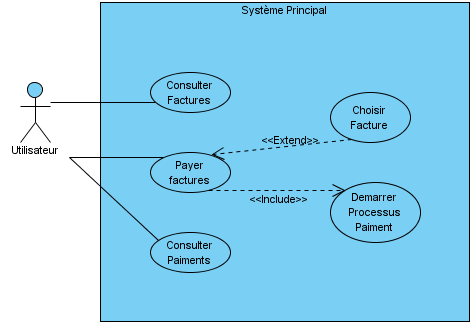
\includegraphics[scale=0.5]{images/uc.png}
		     \end{center}
		     \caption{Diagramme de cas d'utilisation}
		     \label{Diagramme de cas d'utilisation}
	  \end{figure}
	  
	  Pour une premi\`ere utilisation, il est n\'ecessaire de cr\'eer un compte. Les informations \`a fournir sont: un nom, un email, un num\'ero de t\'el\'ephone, la r\'ef\'erence abonn\'ee\footnote{trouver le sens exact} et le mot de passe pour la protection du compte. Ces informations \'etant obligatoires. Un mail d'activation est envoy\'e et l'utilisateur apr\`es activation de son compte peut se connecter \`a l'application. Une authentification est nécessaire afin d'avoir acc\`es aux cas d'utilisations de notre diagramme (ou aux fonctionnalités de l'application).
	  
\subsection{Diagramme de séquence}
 \paragraph{}
	  Le diagramme de séquence représente la succession chronologique des opérations réalisées par un acteur. Ce mode de représentation effectue la description du fonctionnement dynamique du système. En d'autres termes, il indique les objets que l'acteur va manipuler et les opérations qui font passer d'un objet à l'autre.
	  \begin{figure}[H]
		     \begin{center}
			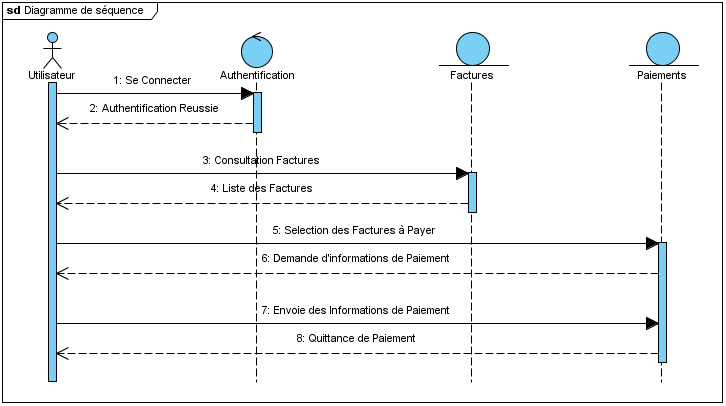
\includegraphics[scale=0.6]{images/sd.png}
		     \end{center}
		     \caption{Diagramme de séquence}
		     \label{Diagramme de cas d'utilisation}
	  \end{figure}
	  Après que l'utilisateur ait entré ses informations, identifiants pour se connecter, il a acc\`es aux factures. L\`a il peut ajouter les factures impay\'ees \`a la liste des factures \`a payer (m\^eme concept que le panier d'un site d'e-commerce). Il pourra donc proc\'eder au paiement de ses factures via le mode de paiement qui lui convient. Une quittance lui est g\'en\'er\'ee et est ajout\'ee \`a son historique de paiements.
   \section{Matériels}
       \subsection{Principe de fonctionnement de notre solution}
      \paragraph{}
	  Nos objectifs pour ce travail sont, dans un premier temps, d'arriver à détecter l'espionnage par webcam et dans un second temps de proposer des options à activer pour protéger l'ordinateur hôte de quelques intrusions qui pourraient survenir. La présentation des principes de fonctionnement se fera en deux étapes: le principe de détection d'attaques par webcam et le principe de protection contre les intrusions.
	  
	  \subsubsection{La webcam}
	  \paragraph{}
	  	Pour détecter l'utlisation illicite d'une ressource, il revient de monitorer en temps réel les flux provenant de cette ressource et générés par des processus. Ainsi, notre solution permet de surveiller les flux de la webcam à intervalles de temps réguliers de trois secondes pour ne pas utiliser, de façon incontrolée, les ressources de l'ordinateur. \\ 
	  	A la découverte d'un processus utilisant la webcam, une alerte est envoyée à l'utilisateur qui choisit si oui ou non il est à la base de l'activité d'un tel processus. Si sa réponse est négative, alors il est victime d'un espionnage et, à ce moment un filtre est fait pour connaitre l'identifiant du processus qui est immédiatement tué. En cas de réponse positive de l'utilisateur (oui c'est bien moi), alors le processus en cours est laissé et la detection de processus utilisant la webcam est désactivée pendant cinq minutes. L'algorithme 1 présente le processus de détection d'espionnage par webcam.
					
%\newpage		
						\begin{algorithm}[H]
						\caption{Algorithme de détection d'espionnage par webcam}
\DontPrintSemicolon % Some LaTeX compilers require you to use \dontprintsemicolon instead

\For{\textit{chaqueTroisSecondes}} {
$etatWebcam \gets enUtilisation()$\;
  \If{$etatWebcam = ouvert$ } {
    $action \gets etesVousAuteur()$\;
     \eIf{$action = non$ } {
    	\textit{chercherIdProcessus()}\;
    	\textit{arreterProcessus()}\;
  }{
	\textit{cinqMinutesDePause()}\;  
  }
  }
}
\Return{$action$}\;
\label{algo:webcam}
\end{algorithm}  		
	  	 
	  	 \subsubsection{Les intrusions }
      \paragraph{}
	   Quand un pirate arrive à prendre possession d'une machine dans un réseau, c'est qu'il est arrivé à établir une connexion entre sa machine et la victime. Ainsi, dans la liste des connexions établies (ESTABLISHED), on peut donc lister la connexion permettant au pirate d'interagir avec sa victime à son insu. Notre solution pour ces attaques est de proposer une option à activer et dont le but est d'alerter l'utilisateur dès qu'une connexion est établie. A cet effet, une vérification des connexions ouvertes se fait toutes les trois secondes. Si l'utilisateur ne reconnait pas cette connexion comme étant légale, alors il le signale par un bouton qu'il appuie et à ce moment, l'adresse source ainsi que le port source de connexion sont mis dans une liste noire. L'algorithme 2 présente les étapes de détection d'intrusions.
	   
	   
						\begin{algorithm}[H]
\DontPrintSemicolon % Some LaTeX compilers require you to use \dontprintsemicolon instead

\For{\textit{chaqueTroisSecondes}} {
$list \gets listeConnexionsEtablies()$\;
	\For{\textit{$connexion$ as $list$}} {
	\textit{alerterConnexionEtablie()}\;
	$action \gets autoriser()$\; 
  \If{$action = non$ } {
   \textit{blacklistAdresseEtPort()}\;
  }
}
}
\Return{$action$}\;
\caption{Algorithme de détection d'intrusions}
\label{algo:intrusion}
\end{algorithm}

Lorsque l'attaque est faite au cours des trois secondes, l'application ne le détecte pas. C'est une de ses faiblesses. 	   
	   \subsubsection{Les whitelist }
      \paragraph{}
	   Il y a des connexions importantes que la machine établit en local avec des adresses locales telle que le 127.0.0.1 qui n'est pas une attaque. Cependant, à l'activation de la détection d'intrusion, notre logiciel alerte l'utilisateur d'une connexion établie en local, ce qui pourrait être considéré comme non importante. C'est ainsi que nous avons proposé une whitelist d'adresses IP où l'utilisateur pourra ajouter ou supprimer les adresses dont il ne s'inquiète pas des connexions établies. Il en est de même pour les ports de connexion tels que le 443 et le 80 qui sont des ports de navigation web. L'utilisateur a donc la possiblité d'ajouter ou de supprimer des ports dans la whitelist, ce qui ne déclenchera plus d'alerte à la découverte d'une connexion avec les paramètres entrés en whitelist. Après avoir modifié la base de données de la whitelist, il faut rafraîchir afin de faire considérer à l'application la nouvelle liste à prendre en compte.
	 	
 		\subsubsection{Les dénis de service}
      \paragraph{}
		Comme nous l'avons présenté au chapitre précédent, un déni de service peut s'effectuer de plusieurs façons. Notre solution, pour cela, propose une option où lorsqu'elle est activée rejette tous les paquets au statut invalide et les paquets avec tous les flags activés (XMAS). Aussi limite-elle le nombre de paquets ICMP à deux (02) par seconde pour eviter les attaques de type Smurf.   
     
	\subsubsection{Limiter le nombre de connexion par adresse}
      \paragraph{}
     Toujours dans l'optique d'arriver à une fin de déni de service, l'attaquant peut falsifier les adresses IP et envoyer des demandes de connexion, la cible peut se retrouver avec une immensité de connexions ouvertes pour une seule adresse. Pour eviter cela, nous proposons à l'utilisateur d'entrer le nombre de connexions maximales qu'il admet pour une adresse IP vers sa machine en dépendance des services qu'il fournit au réseau auquel il appartient. Une fois cette valeur entrée et validée, une règle est créée pour rejeter toute demande de connexion d'une quelconque adresse après avoir atteint la limite entrée par l'utilisateur. Ce dernier a la possibilité de modifier cette valeur à tout moment.    
  \subsection{Langage de développement et outils}
  
      \paragraph{}
	  Notre solution fonctionne sous les systèmes Linux. Cette plate-forme a été choisie en raison de son ouverture, de l'accessibilité au code source et de sa flexibilité. Pour atteindre nos objectifs, nous avons utilisé les langages java, awk et bash; les deux derniers étant des langages de script de Linux. Il est à noter que les versions Debian sont les plus concernées par notre travail. Le tableau suivant fait la synthèse des outils utilisés.
	  
	\begin{table}[H]
	   \begin{center}
	      \caption{Synthèse des outils utilisés}
	      \label{Synthèse des outils utilisés}
		\begin{tabular}{|>{\centering\arraybackslash} p{5cm} |>{\centering\arraybackslash} p{5cm}|>{\centering\arraybackslash} p{5cm}|}
		 \hline
		\begin{bf}Langages\end{bf} & \begin{bf} Systèmes d'exploitation\end{bf} & \begin{bf}Autres Outils \end{bf}\\
		\hline
		\multicolumn{1}{|l|}{Java } & \multicolumn{1}{|l|} {Ubuntu 16.04 LTS}& \multicolumn{1}{|l|}{Iptables }\\
		\hline
		\multicolumn{1}{|l|}{Bash } & \multicolumn{1}{|l|} {Kali Linux 2.0 Rolling}& \multicolumn{1}{|l|}{ }\\
		\hline
		\multicolumn{1}{|l|}{Awk} & \multicolumn{1}{|l|}{} & \multicolumn{1}{|l|}{ }\\
		\hline
		
		\end{tabular}
	   \end{center}
	  \end{table}
	  
	 Les langages et outils présentés dans le tableau sont ceux utilisés pour le développement de notre application pendant que les systèmes d'exploitations présentés sont ceux utilisés pour le cas pratique.

      \subsection{A propos de Debian}
	\paragraph{}
	  Debian est un système d'exploitation libre. Il est simple et est constitué de plus de 4000 paquets. Les paquets sont des composants logiciels précompilés conçus pour s'installer facilement sur la machine hôte. L'ouverture de Debian permet à plusieurs programmeurs de pouvoir identifier les failles de sécurité ou de créer plusieurs modules pour faire des tâches qui s'avèrent indispensables. C'est ainsi que la communauté de Debian devient de plus en plus robuste et flexible. Plusieurs systèmes d'exploitation sont dérivés de Debian dont Kali Linux spécialisé dans les tests d'intrusion. 
  
\section*{Conclusion}
		\paragraph{}
	  Dans ce chapitre, nous avons présenté les choix techniques opérés
	  ainsi que notre solution à travers sa modélisation, son principe de fonctionnement et les outils utilisés. 
	  Le chapitre suivant exposera les différents résultats et quelques critiques.

\chapter{Résultats et Discussion}\label{chap:3}
   \section*{Introduction}
    \paragraph{}
    Dans ce chapitre, nous présentons les résultats des simulations faites pour tester le fonctionnement de notre solution. Dans un premier temps,
    nous allons présenter l’application, une attaque pour tester la s\'ecurit\'e de notre r\'eseau et nous aborderons ensuite une discussion.


    \section{Présentation des résultats des tests}
      \paragraph{}
	  \begin{figure}[H]
	      \begin{center}
		  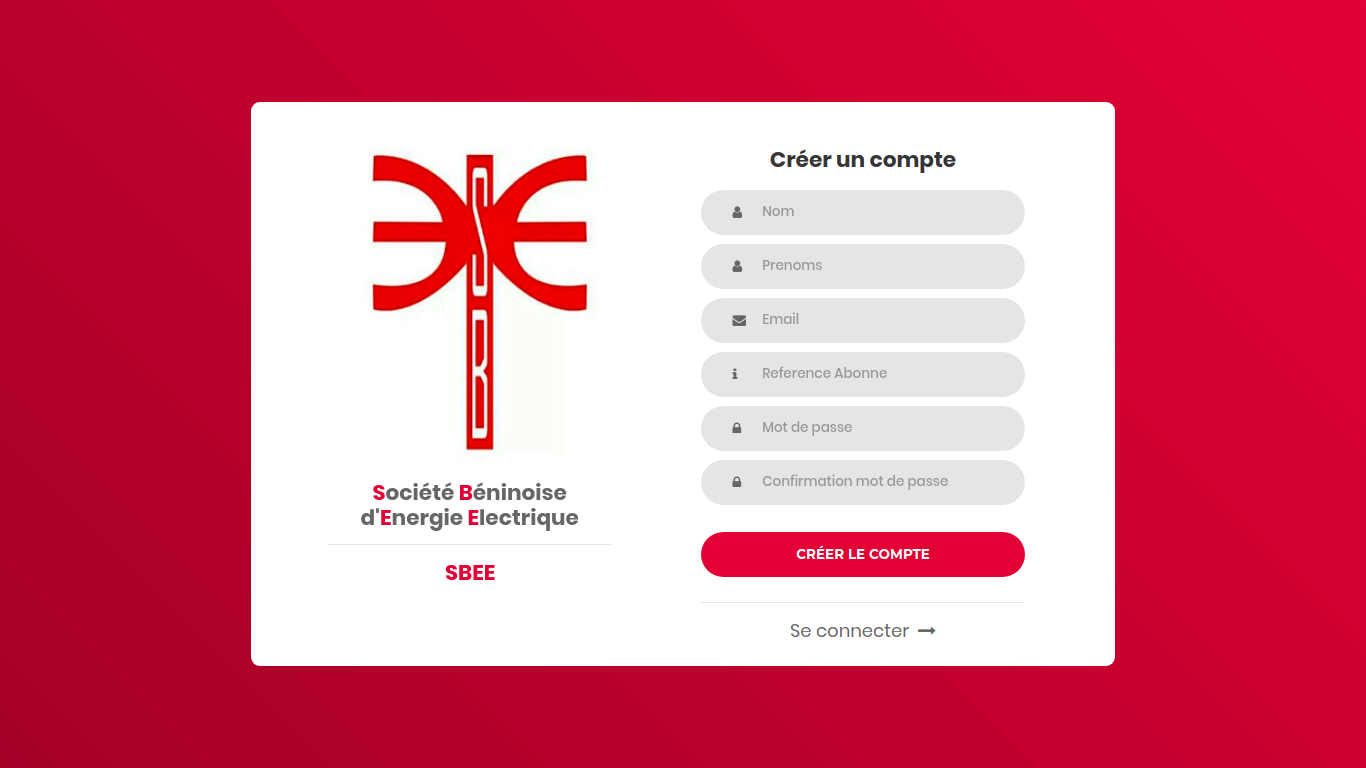
\includegraphics[scale=0.35]{images/register.png}
	      \end{center}
	      \caption{Page d'inscription de l'application}
	      \label{Accueil}
	  \end{figure}
	  La figure 3.1 présente la page d'ouverture de compte de notre application. L'utilisateur entre son nom, pr\'enom(s), adresse email, la r\'ef\'erence abonn\'ee et le mot de passe. Un mail d'activation lui est envoy\'e et il est redirig\'e vers la page de connexion.
	      
	  \begin{figure}[H]
	      \begin{center}
		  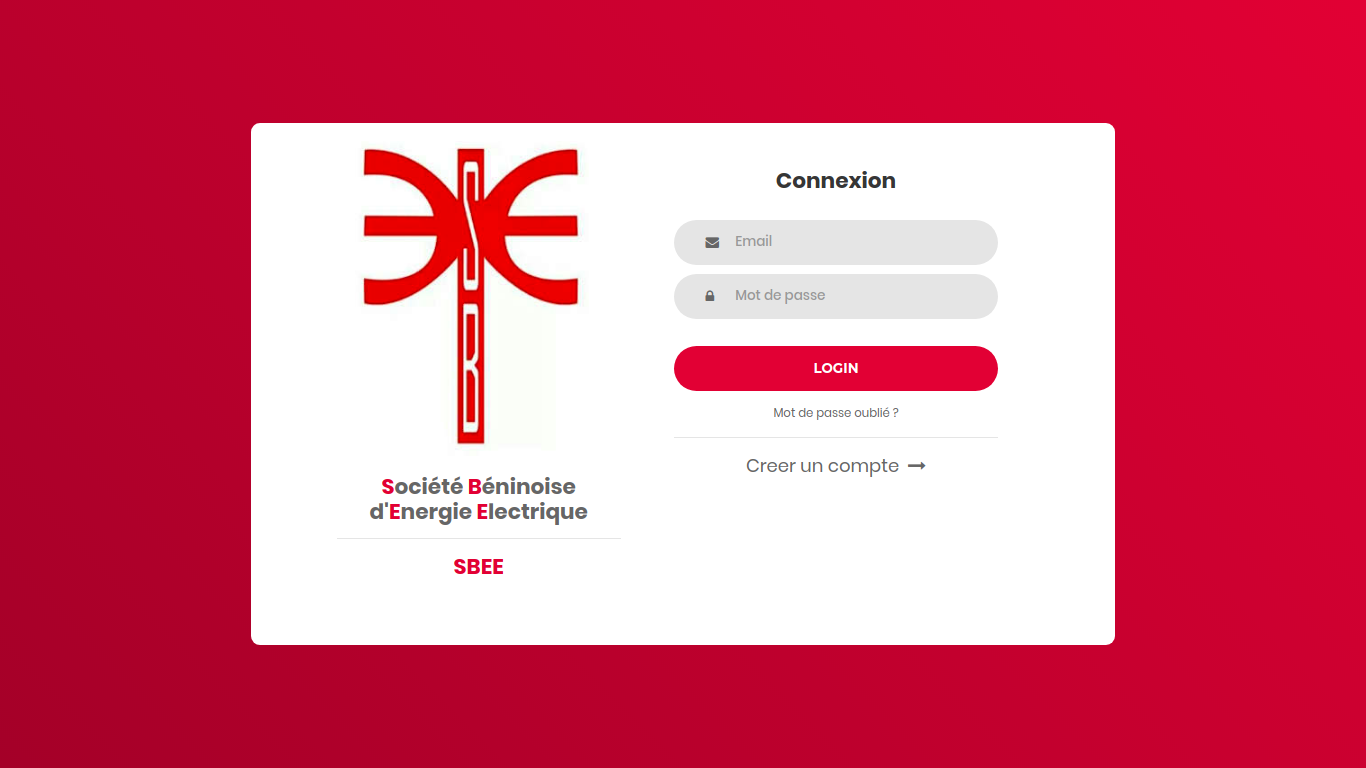
\includegraphics[scale=0.35]{images/login.png}
	      \end{center}
	      \caption{Page de connexion}
	      \label{Page de la whitelist IP}
	  \end{figure}
	  L'utilisateur entre son email et son mot de passe pour se connecter \`a l'application.
      
      \subsection{Interfaces Abonn\'e}
	  \begin{figure}[H]
	      \begin{center}
		  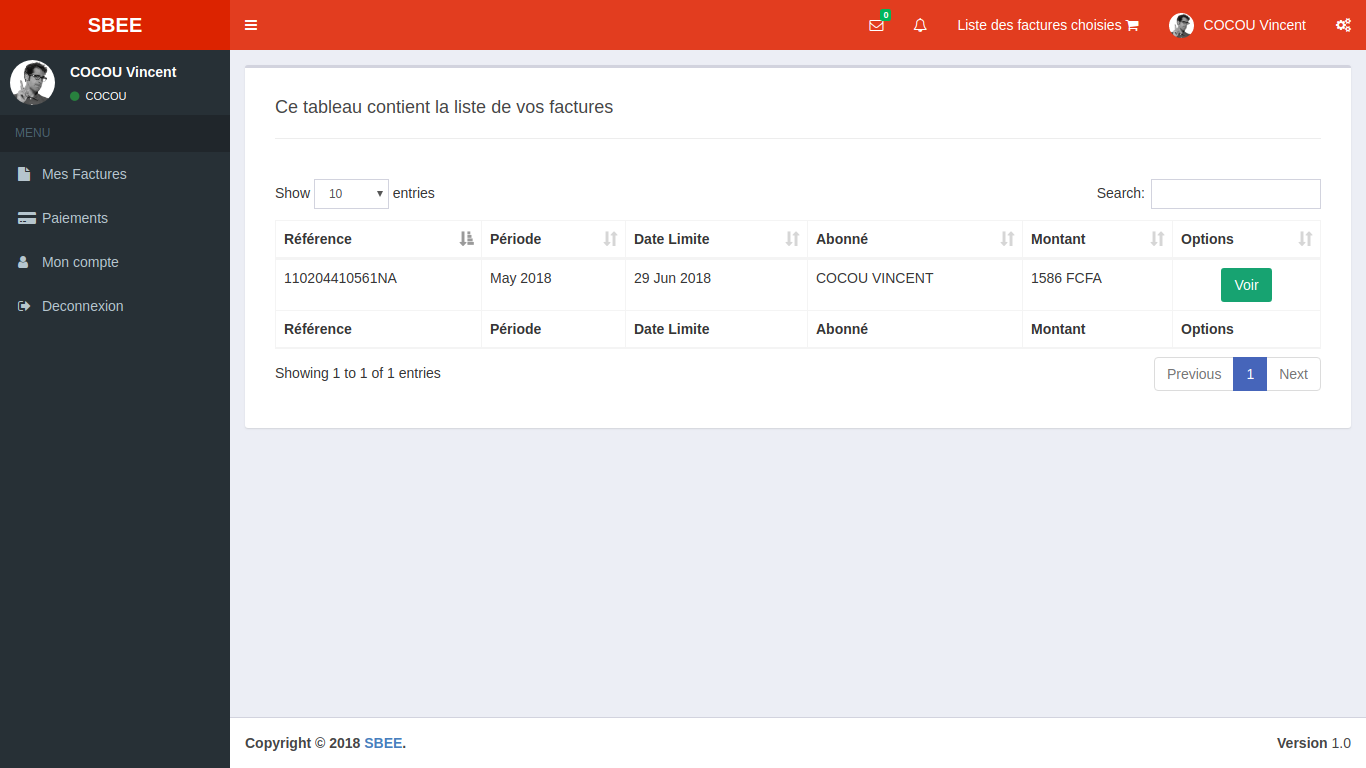
\includegraphics[scale=0.35]{images/listfactures.png}
	      \end{center}
	      \caption{Liste des factures de l'abonn\'e}
	      \label{Page de la whitelist Port}
	  \end{figure}
	  Tous les utilisateurs ont acc\`es \`a la liste de leurs factures. Ils peuvent cliquer sur le bouton \textbf{Voir} pour voir la facture sous le format habituel qu'ils connaissent (le format d'impression et de distribution), ou juste afficher les informations sous forme de liste.
			      
	  \begin{figure}[H]
	      \begin{center}
		  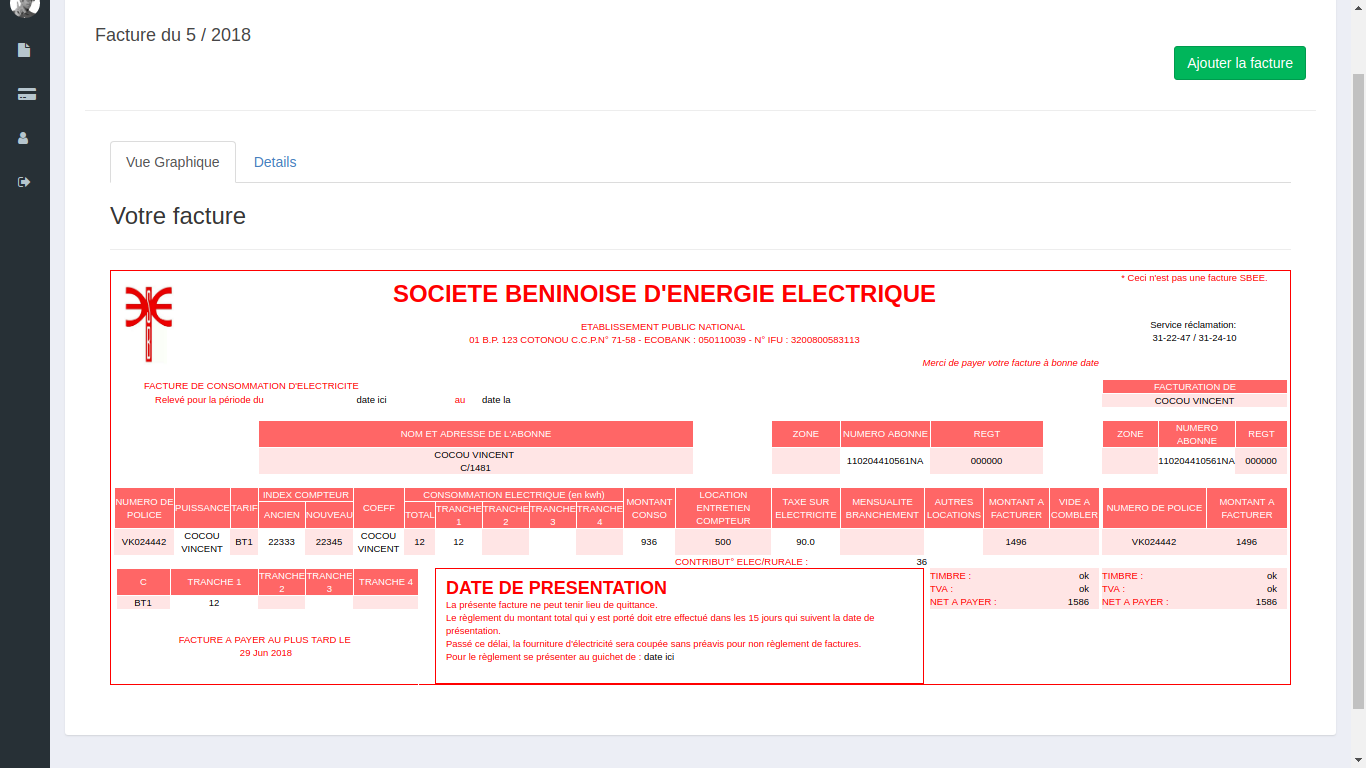
\includegraphics[scale=0.35]{images/graphic.png}
	      \end{center}
	      \caption{Vue d'une facture (Format d'impression)}
	      \label{Page de la whitelist Port}
	  \end{figure}
	  Il s'agit d'une repr\'esentation de la facture physique que nous connaissons tous.
						      
	  \begin{figure}[H]
	      \begin{center}
		  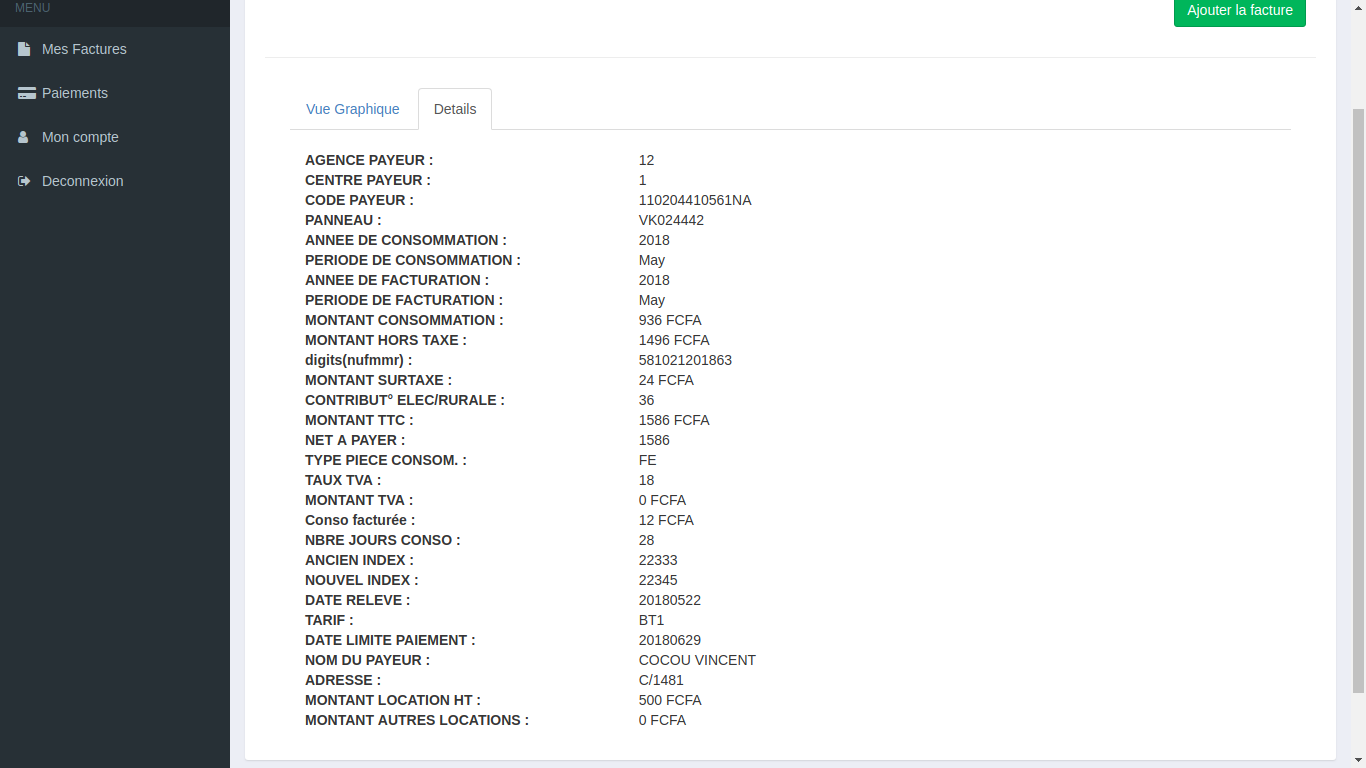
\includegraphics[scale=0.35]{images/details.png}
	      \end{center}
	      \caption{Vue d'une facture (Liste d'informations)}
	      \label{Page de la whitelist Port}
	  \end{figure}
	  Ce format permet d'avoir les informations d'une fa\c{c}on plus lisible et plus claire.
			      
	  \begin{figure}[H]
	      \begin{center}
		  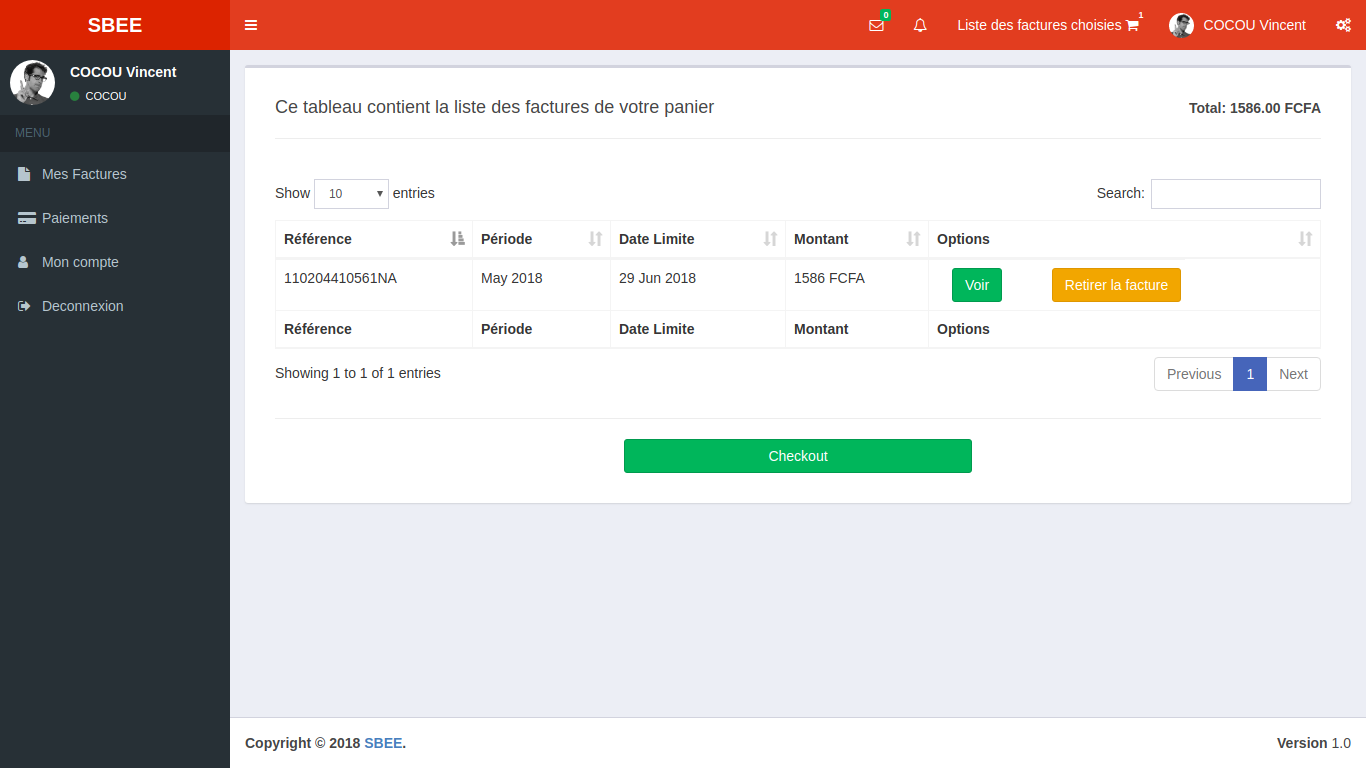
\includegraphics[scale=0.35]{images/choix.png}
	      \end{center}
	      \caption{Liste des factures choisies}
	      \label{Page de la whitelist Port}
	  \end{figure}
	  Afin de permettre de solder plusieurs factures en une fois, l'utilisateur choisit toutes les factures qu'il d\'esire r\'egler et ensuite il proc\`ede au checkout\footnote{Expression anglaise: régler la note, proc\'eder au paiement}.
			      
	  \begin{figure}[H]
	      \begin{center}
		  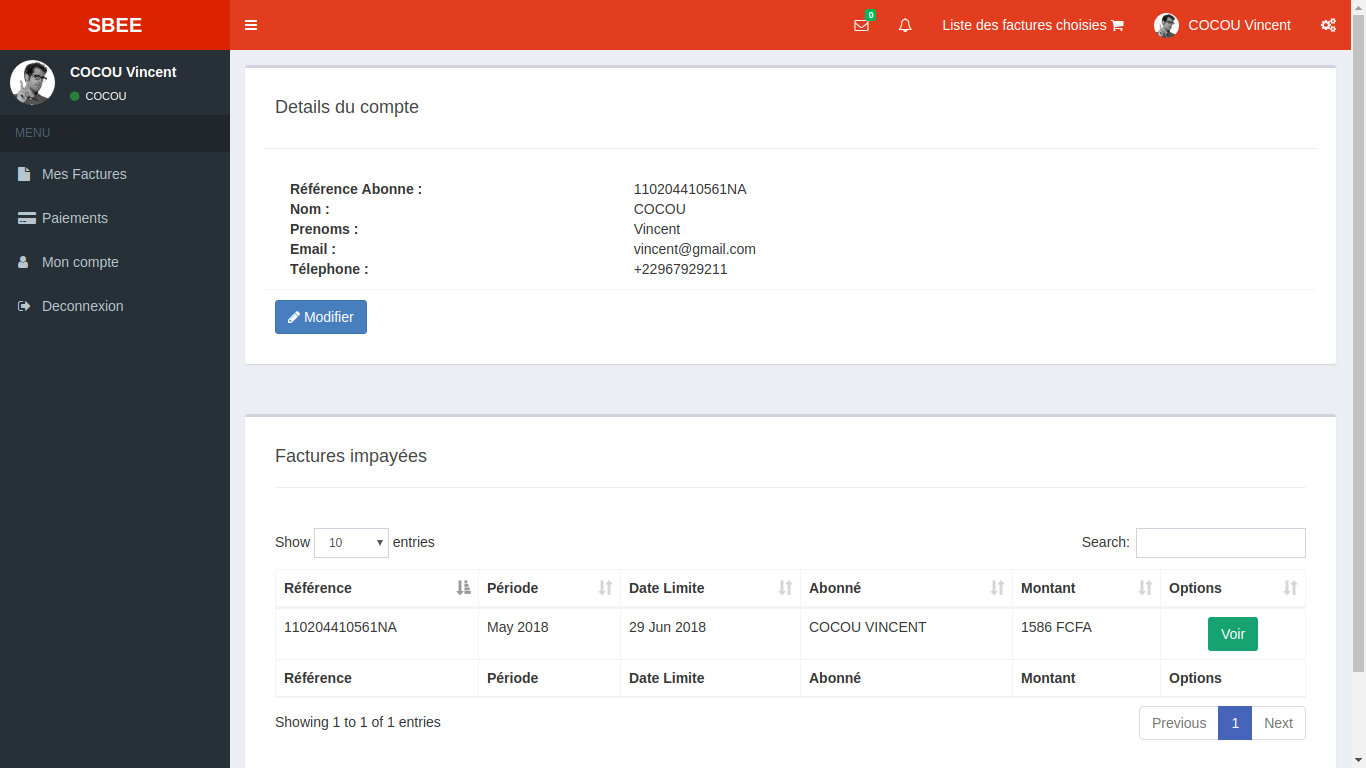
\includegraphics[scale=0.35]{images/detailcompte.png}
	      \end{center}
	      \caption{Le compte d'un utilisateur}
	      \label{Page de la whitelist Port}
	  \end{figure}
	  L'utilisateur a acc\`es aux informations de son compte. Et il peut actuellement modifier son nom, pr\'enom et num\'ero de t\'elephone.
		
      \subsection{Interfaces Administrateurs}
	 Les Administrateurs ont acc\`es \`a bien plus de fonctionnalit\'es que les abonn\'es simples:
	  \begin{itemize}
	    \item La liste des utilisateurs de la plateforme (abonn\'es simples et administrateurs)
	       \begin{figure}[H]
		  \begin{center}
		      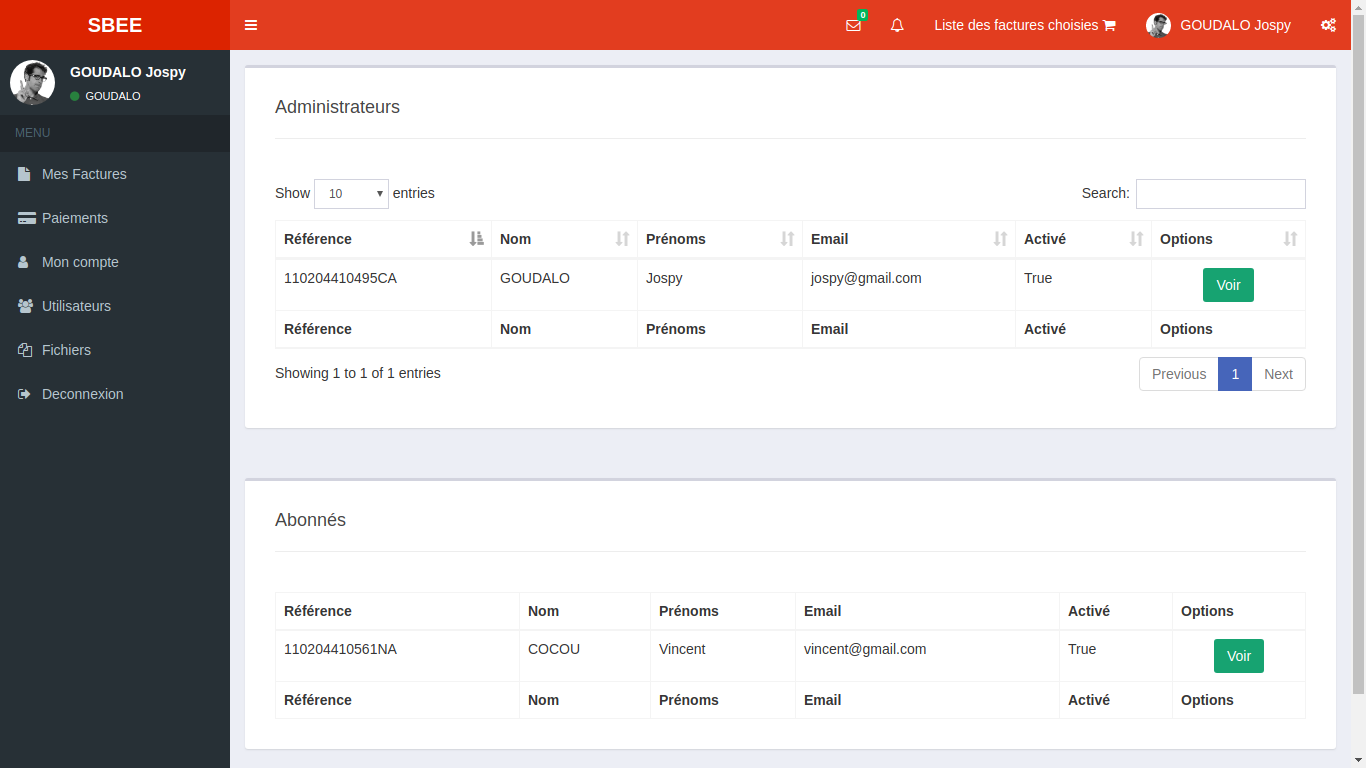
\includegraphics[scale=0.35]{images/gcv.png}
		  \end{center}
		  \caption{Utilisateurs de la plateforme}
		  \label{Page de la whitelist Port}
	      \end{figure}
	    
	    \item Les fichiers: la liste de tous les fichiers factures charg\'es dans la base de données ainsi que les r\`eglements,
	      \begin{figure}[H]
		  \begin{center}
		      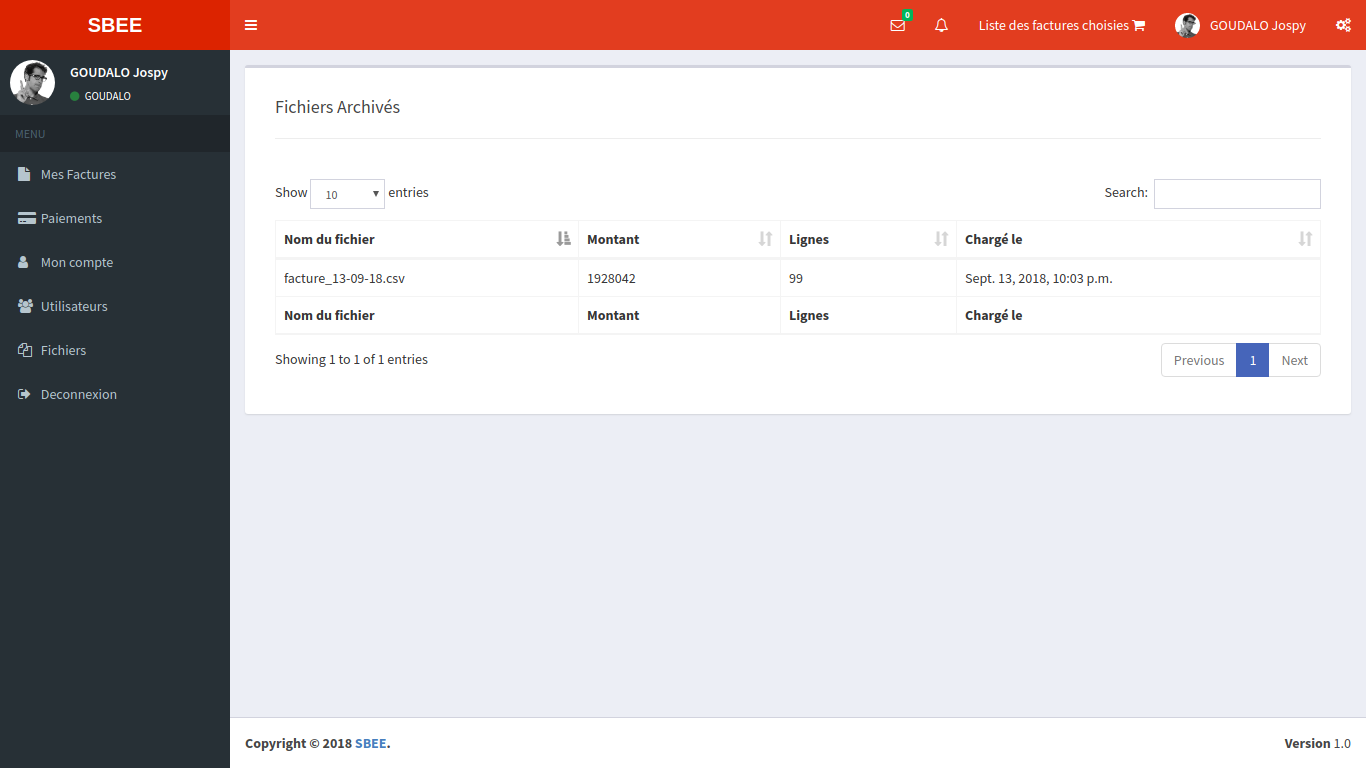
\includegraphics[scale=0.35]{images/files.png}
		  \end{center}
		  \caption{Fichiers import\'es}
		  \label{Page de la whitelist Port}
	      \end{figure}
	      
	  \end{itemize}

	      
    \section{Discussion}
	  \paragraph{}
	      Notre projet est né de plusieurs constats dont entre autre les pertes de temps dans les guichets de la SBEE, et les multiplications croissantes des attaques et intrusions informatiques. Des travaux n'ont pas encore \'et\'e faits \`a l'interne dans les locaux de la SBEE pour palier \`a ces probl\`emes observ\'es. Ceci repr\'esente donc un premier pas fait vers le paiement des factures num\'eriques.
	      
	  \paragraph{}
	      Ainsi, d'une part, notre solution est simple à utiliser et est utilisable depuis un navigateur web. Elle est accessible via internet et ne requiert aucun équipement ou installation spécifique chez l'utilisateur. Elle permet aux utilisateurs de consulter leurs factures et ainsi donc de suivre leur consommation plus facilement. Cependant la soci\'et\'e choisira elle-m\^eme via un appel d'offre ses prestataires pour les diff\'erentes solutions de paiement. Nous avons eu \`a faire quelques recommandations dont: \textbf{Mobile Money de MTN} ainsi que le service mondialement reconnu \textbf{PayPal}.
	      
	  \paragraph{}
	      Aussi existe-t-il des risques de double paiements lors des factures. Etant donn\'e que Gd'Or fonctionne en mode non connect\'e et que les factures ne sont valid\'ees qu`apr\`es 00h, un utilisateur qui va en agence pourrait payer une facture qui a d\'ej\`a \'et\'e pay\'ee en ligne. Cependant ces cas seront rembours\'es par les acteurs des diff\'erentes solutions de paiement car Gd'Or d\'etecte automatiquement les doublures lors de l'apurement des comptes et renvoie des fichiers contenant les erreurs aux entit\'es correspondantes. Celle derni\`ere proc\'edera \`a un remboursement des fonds aux utilisateurs concern\'es.

	  \paragraph{}
	      D'autre part, l'architecture et les outils propos\'es nous permettent d'assurer un minimum de s\'ecurit\'e pour notre application et dans notre r\'eseau. Notre strat\'egie se base essentiellement sur la maitrise du flux de donn\'ees et de la connaissance effective de chaque entit\'e du r\'eseau. Et ceci est un prérequis pour assurer la sécurité : \textbf{On ne protège bien que ce que l’on connaît}. Cependant cette architecture ne nous met pas à l’abri de toutes les attaques, mais nous prot\`ege quand m\^eme contre beaucoup d'attaques courantes, ce qui n’est pas négligeable.

	      
    \section*{Conclusion}
	  \paragraph{}
		  Dans ce chapitre, nous avons exposé les résultats des tests de notre application et réalisé quelques critiques concernant ses performances et ses insuffisances. Ces insuffisances peuvent être perçues comme des perspectives afin d'améliorer le travail fait pour une utilisation plus efficiente.

 %\include{perspectives}
%conclusion
\conclusion
\conclusion
		\paragraph{}
			La sécurité informatique passant par la sécurité de l'information, la sécurité de la vie privée n'est plus aujourd'hui un sujet inconnu. Aussi le hacking constitue-t-il aujourd'hui une arme de guerre assez dévastatrice et silencieuse. Dans cette vision, beaucoup d'outils de sécurité se développent de jour en jour afin de restreindre le champ d'attaque des pirates informatiques qui s'arment davantage. 
		\paragraph{}
			L'objet de ce mémoire a été de mettre en place un système de détection des attaques par webcam et de prévenir par des moyens simples mais efficaces les tentatives d'intrusion. Les solutions proposées proviennent des analyses éffectuées sur les systèmes piratés volontairement. Ainsi les utilisateurs de notre application peuvent être protégés des différentes menaces que nous couvrons.
		\paragraph{}
			Dans ce mémoire, nous avons tout d'abord fait une revue de littérature autour des intrusions informatiques. Nous avons ensuite réalisé la conception de la solution que nous avons proposée avant d'exposer les résultats
			et critiques de l'application que nous avons implémentée.
		\paragraph{}
			Bien que notre solution réponde au besoin énoncé, il faut noter certaines insuffisances telles que 
			l'inactivité de l'application dans les intervalles d'attente.  Bien que cela soit fait pour éviter l'utilisation abusive des ressources du système, il serait préférable de mettre le système en mode écoute. D'une part, un autre axe
			de recherche en ce qui concerne les travaux futurs sera d'explorer la possibilité de rendre 
			l'application accessible sur d'autres plateformes telles que Windows, MAC OS et toutes autres distributions Linux. D'autre part, on pourrait envisager de mettre la recherche de symptômes d'attaques en mode écoute en prenant des mesures autonomes. \cite{ehrig2006graph}

\lhead[]{} \rhead[]{} \chead[]{}

%%biblio
%\addcontentsline{toc}{chapter}{Bibliographie}
%\bibliographystyle{abbrv}
%\bibliography{biblio/biblio}

\begin{thebibliography}{9}\addcontentsline{toc}{chapter}{Bibliographie}
 
\bibitem{b} Le petit Larousse Illustré 2010

\bibitem{c}
Patrcick Engebretson, "Les bases du hacking", Pearson 2013	

\bibitem{d}
Kerry Cox, Christopher Gerg, "Sécurité réseau avec Snort et les IDS"  O'Reilly 2004	
    
\bibitem{E}
David Kennedy, Jim O'Gorman, Devan Kearns et Mati Aharoni "Hacking, Sécurité et tests d'intrusion avec Métasploit", Pearson 2013

\bibitem{i}
Jesse Russell and Ronald Cohn , "Fail2ban", Book on Demand 2012

\bibitem{I}
Alexandre Gachet, "Introduction à UML", O'Reilly 2005

\chapter*{Webographie}
\addcontentsline{toc}{chapter}{Webographie}

\bibitem{rpg}
RPG, \url{https://search400.techtarget.com/definition/Report-Program-Generator}, consulté le 29 Juillet 2017

\bibitem{A}
Larousse, \url{http://www.larousse.fr/dictionnaires/francais/hacker/38812}, consulté le 28 Mai 2017

\bibitem{momo}
MoMo API - MTN B\'enin, \url{https://www.mtn.bj/particuliers/mobile-money/momo-api/}, consulté le 08 Août 2018

\bibitem{paypal}
Paypal, \url{https://www.paypal.com}, consulté le 08 Août 2018

\bibitem{nginx}
Nginx, \url{http://www.aosabook.org/en/nginx.html}, consulté le 22 Août 2018

\bibitem{iptables}
Iptables, \url{https://blog.microlinux.fr/iptables/}, consulté le 20 Août 2018

\bibitem{samba}
Samba, \url{https://openclassrooms.com/fr/courses/2929586-mettre-en-place-un-serveur-samba}, consulté le 02 Septembre 2018

\bibitem{ranking}
W3techs, \url{https://w3techs.com/technologies/cross/web_server/ranking}, consulté le 02 Septembre 2018

\end{thebibliography}



\chapter*{Annexe}\addcontentsline{toc}{chapter}{Annexe}\label{annexe1}

\subsection*{Étapes clés du déroulement de l'attaque}


Nous allons exploiter quelques failles de ce réseau pour effectuer une attaque man in the middle (MITM).\\

Au début, notre machine Windows peut atteindre normalement le routeur R4.
\begin{figure}[H]
    \centering
    \includegraphics[scale=0.8]{images/ping_b4_1}
    \caption{Ping vers le routeur R4 avec succès}
    \label{fig:ping_b4_1}
\end{figure}
Quand on essaie de tracer le chemin vers R4, on constate que la machine passe par le routeur R1 légitime du lien pour atteindre R4
\begin{figure}[H]
    \centering
    \includegraphics{images/tracert_b4_1}
    \caption{Traces du chemin vers R4}
    \label{fig:tracert_b41}
\end{figure}
L'attaquant sur le lien peut alors passer a l'attaque.
Pour effectuer l'attaque MITM on utilisera l'outil fake\_router6, un utilitaire du package d'outils \textbf{the hacker choice}.
Ainsi sur la machine d'attaque, on active en un premier lieu le forwarding pour être transparent et ne pas bloquer le transit des paquets.
\begin{figure}[H]
    \centering
    \includegraphics{images/attk/fwrd_activation}
    \caption{Activation du forwarding des paquets.}
    \label{fig:activ_fwrd}
\end{figure}
Aussi on lance wireshark pour observer le trafic des paquets sur notre interface dans le réseau.\\
-------\\
Puisque tout est prêt nous allons lancer l'attaque.

\begin{figure}[H]
    \centering
    \includegraphics[scale=0.8]{images/attk/lancement_attk_1}
    \caption{Initialisation de l'attaque}
    \label{fig:attk_init_1}
\end{figure}

L'attaque est en cours et l'attaquant s'annonce comme le routeur par défaut du lien
nous allons maintenant vérifier la table des routes de notre machine windows.
\begin{figure}[H]
    \centering
    \includegraphics{images/attk/tableRoutes_windows}
    \caption{Table des routes de la machine victime}
    \label{fig:win_route_table}
\end{figure}
On constate que l'attaquant s'est insère comme passerelle de la victime.
pour confirmer cela reprenons un tracert vers le routeur r4
\begin{figure}[H]
    \centering
    \includegraphics{images/attk/tracert_b4_2}
    \caption{Chemin vers b4 pendant l'attaque.}
    \label{fig:tracert_b42}
\end{figure}
On peut voir clairement que la victime passe par l'attaquant pour atteindre le routeur.\\

A présent nous allons essayer de capturer une information envoyée par la victime.
Pour cela la victime fait un telnet sur le router R4 pour s'y connecter avec les paramètres suivants:\\
password1:\textbf{cisco}\\
password2:\textbf{class}
\begin{figure}[H]
    \centering
    \includegraphics{images/attk/telnet_r4}
    \caption{Connexion telnet au routeur.}
    \label{fig:telnetr4}
\end{figure}

Une fois la connexion réussie, nous allons voir avec wireshark les paquets de connexion et y retrouver les paramètres de connexion.
\begin{figure}[H]
    \centering
    \includegraphics[width=1.0\textwidth]{images/attk/c}
    \includegraphics[width=1.0\textwidth]{images/attk/i}
    \includegraphics[width=1.0\textwidth]{images/attk/s}
    \includegraphics[width=1.0\textwidth]{images/attk/c2}
    \includegraphics[width=1.0\textwidth]{images/attk/o}   
    \caption{Premier paramètre de connexion au routeur R4: \textbf{c-i-s-c-o}}
    \label{fig:param_conn_r4}
\end{figure}
\begin{figure}[H]
    \centering
    \includegraphics[width=1.0\textwidth]{images/attk/param2_c}
    \includegraphics[width=1.0\textwidth]{images/attk/param2_l}
    \includegraphics[width=1.0\textwidth]{images/attk/param2_a}
    \includegraphics[width=1.0\textwidth]{images/attk/param2_s1}
    \includegraphics[width=1.0\textwidth]{images/attk/param2_s2}
    \caption{Second paramètre de connexion au routeur R4: \textbf{c-l-a-s-s}}
    \label{fig:param_conn2}
\end{figure}
Les paramètres on été retrouves donc l'attaque a été un succès!

%\subsection*{Mitigations}
%Pour sécuriser ce réseau afin d'éviter ce genre d'attaque, deux mesures de sécurité peuvent être configurées.
%\begin{itemize}
%    \item le SEND
%    \item le RaGuard
%\end{itemize}


\end{document}
